\documentclass[onside]{book}
\usepackage{lmodern}
\usepackage[T1]{fontenc}
\usepackage{mathtools}
\usepackage{hyperref}
\usepackage{amsmath}
\usepackage[catalan]{babel}
\usepackage{lipsum}  
\usepackage[Lenny]{fncychap}
\usepackage{multirow}
\usepackage{graphicx,wrapfig}
\usepackage{xcolor}
\usepackage{fancyhdr}
\usepackage{inputenc}
\usepackage{geometry}
\usepackage{enumitem}
\usepackage{caption}
\usepackage{subcaption}
\usepackage{footnote}
\usepackage{tabularx}
\ChNameVar{\fontsize{20}{60}\selectfont\fontseries{bx}\fontfamily{cmr}}
\ChNumVar{\fontsize{50}{100}\selectfont\fontfamily{cmr}}
\pagestyle{fancy}
\geometry{a4paper,left=25mm,right=25mm,headheight=2.5cm, bottom=2.5cm}
\addtolength{\textheight}{-60pt}
\usepackage{imakeidx}
\renewcommand{\headrulewidth}{0pt}
\usepackage{makecell}
\renewcommand\theadalign{bc}
\renewcommand\theadfont{\bfseries}
\renewcommand\theadgape{\Gape[4pt]}
\renewcommand\cellgape{\Gape[4pt]}
\makesavenoteenv{tabular}
\makesavenoteenv{table}
\usepackage{titlesec}
%\pagenumbering{arabic}
%\fancyfoot[R]{\thepage}

\fancyhead{}
\renewcommand{\contentsname}{\Large{\sffamily\textbf{Índice}}}
\begin{document}
\renewcommand{\headrulewidth}{0pt} %No Horizontal Line at top
%\newcommand*\NewPage{\clearpage\thispagestyle{empty}\null} 

\begin{figure}[hbt!]

\includegraphics[width=6.5cm]{logo.pdf}
\end{figure}
\fontfamily{qhv}\selectfont
\vspace{13mm}
\begin{flushleft}
\hspace{10mm}\LARGE{\textbf{TREBALL DE FI DE GRAU}}\\
\end{flushleft}
\vspace{19mm}
\begin{flushright}
\LARGE{\textbf{ONES MAGNETOHIDRODINÀMIQUES EN UN MEDI\\
\hspace{1cm}
ACOTAT USANT DEDALUS}}\\
\end{flushright}
\vspace{30mm}
\begin{flushleft}
\hspace{10mm}\LARGE{\textbf{Joan Ribot Oliver}}\\
\vspace{11mm}
\hspace{10mm}\large{\textbf{Grau de {Física}}}\\
\vspace{7mm}
\hspace{10mm}\large{\textbf{Facultat de Ciències}}\\
\vspace{20mm}
\hspace{10mm}\normalsize{\textbf{Any Acadèmic 2024-25}}
\end{flushleft}
\thispagestyle{empty}
\newpage
\thispagestyle{empty}
\mbox{}
\newpage
%========================================================
\begin{figure}[hbt]
\thispagestyle{empty}
\end{figure}
\begin{flushleft}
\hspace{1cm}
\LARGE{\textbf{ONES MAGNETOHIDRODINÀMIQUES EN UN MEDI\\
\hspace{1cm}
ACOTAT USANT DEDALUS}}\\
\vspace{29mm}
\hspace{10mm}\LARGE{\textbf{Joan Ribot Oliver}}\\
\vspace{7mm}
\hspace{1cm}\LARGE{\textbf{Traball de Fi de Grau}}\\
\vspace{7mm}
\hspace{1cm}\Large{\textbf{Facultat de Ciències}}\\
\vspace{7mm}
\hspace{1cm}\Large{\textbf{Universitat de les Illes Balears}}\\
\vspace{7mm}
\hspace{1cm}\normalsize{\textbf{Any Acadèmic 2024-25}}\\
\vspace{17mm}
\hspace{1cm}\small{Paraules claus del treball:}\\
\vspace{3mm}
\hspace{1cm}\small{autofuncions, mode/s, Alfvén, ràpids, lents, dispersió}\\
\vspace{25mm}
\hspace{1cm}\large{\textit{Nom Tutor/Tutora del Treball: Ramon Oliver Herrero}}\\
\vspace{1cm}
\end{flushleft}
\fancypagestyle{footer}{\fancyfootoffset[L]{-0.9cm}\fancyfootoffset[R]{-0.9cm}\fancyhf{}\lfoot{
  \makebox[\dimexpr\textwidth-2\fboxsep-2\fboxrule\relax]{%
  \parbox[b]{3.8in}{\fontfamily{qhv}\selectfont Autoritz la Universitat a incloure aquest treball en el repositori institucional per consultar-lo en accés obert i difondre'l en línia, amb finalitats exclusivament acadèmiques i d'investigació.}\hspace{1.9cm}
  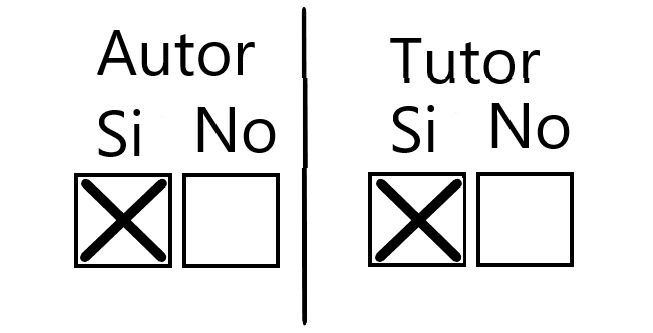
\includegraphics[scale=0.2]{tik_cross_blank_cat_si.png}
  
}}}

\thispagestyle{footer}
\newpage
\thispagestyle{empty}
\mbox{}
\newpage
%====================================
{\fontfamily{cmr}\selectfont
     \noindent\Large{\sffamily\textbf{Resum}}\\
     
    \normalsize{
    Les protuberàncies o prominències solars són un dels fenòmens més rellevants i freqüents en l'atmosfera solar.
    Aquestes es troben envoltades per la corona solar, la capa més calenta, externa i lleugera del sol.
    Les protuberàncies són més denses i fredes que aquesta i poden romandre en equilibri quiescent durant períodes de díes a setmanes.
    Sobre l'estat estacionari hi apareixen petites oscil·lacions que recorden els modes normals d'una corda amb els extrems fixats.
    S'aproxima el sistema com una làmina infinita amb un camp magnètic horitzontal,
    de manera que s'estudien les variacions de la prominència en aquesta situació.
    Les equacions de la magnetohidrodinàmica (MHD) són resoltes, es proposen solucions com a ones planes i el problema es desacobla en dos subconjunts d'equacions:
    les dels modes d'Alfvén i les dels modes ràpids i lents.
    S'analitzen i es classifiquen els modes resultants segons la seva estructura, localització i relació de dispersió.
    Els resultats mostren encreuaments evitats i acoblaments entre modes, de manera que s'obté una descripció qualitativa de les oscil·lacions estacionàries en plasmes solars.
    Tot això es realitza mitjançant un codi numèric en llenguatge Python i amb l'ajuda de la llibreria Dedalus, especialitzada en resoldre equacions diferencials parcials (PDE).

    % En toodels ho fa molt bé es cabró!
    %Les protuberàncies solars són estructures denses i fredes que es mantenen en equilibri dins la corona solar, una regió calenta i difusa de l'atmosfera del Sol.
    %En aquest treball s’estudia la propagació d’ones magnetohidrodinàmiques (MHD) en una protuberància quiescent mitjançant el codi numèric Dedalus,
    %resolent les equacions MHD sota condicions físiques simplificades.
    %El sistema s’aproxima com una làmina plana amb condicions de contorn als extrems i un camp magnètic horitzontal constant.
    %S’analitzen els modes normals que s’hi poden excitar —modes d’Alfvén, ràpids i lents— i es classifiquen segons la seva estructura (fonamental o harmònica),
    %localització (interna, externa o híbrida) i resposta en funció del vector d’ona.
    %Els resultats mostren acoblaments entre modes i encreuaments evitats, aportant una visió quantitativa de les oscil·lacions estacionàries en plasmes solars.
    } \\
    
    \noindent\Large{\sffamily\textbf{Resumen}}\\

    
    \normalsize{
    \lipsum[1-1]} \\
    
    \noindent\Large{\sffamily\textbf{Abstract}}\\

    
    \normalsize{
      Magnetohydrodinamical waves with boundary conditions using Dedalus

This repo is about my final graduate project at Universitat de les Illes Balears (UIB). It contains some python notebooks including the ones to test and learn how to use the Dedalus library.

The main goal of this project is to learn and take advantage of this useful tool to solve the PDE obtained with the linearization of the equations of ideal MHD, among some other assumptions described in the memory of the project.

This equations represent the dynamics of the normal modes of a wave propagating in a solar prominence at the solar corona, which conforms a 3D bounded system. However, there are two sets of equations which are uncoupled and can be separated by three modes: the Alfvén modes, which propagate just as a guitar string with non continous density (1D), and the Fast & Slow modes, which couple the movement in the two remaining dimensions.
    \lipsum[1-1]}\\

\thispagestyle{empty}
\let\cleardoublepage\clearpage
\tableofcontents
\addtocontents{toc}{\vspace{-2cm}}
\thispagestyle{empty}
\let\cleardoublepage\clearpage
{\fontfamily{cmr}\selectfont
%\thispagestyle{empty}


\chapter{Introducció}

EL QUE HE PUC FER PERQUÈ L'ÍNDEX QUEDI BÉ ÉS AFEGIR TOTES LES CAPÇALERES (SECCIONS, SUBSECCIONS, ETC.) EN AQUEST .TEX I DESPRÉS TALLAR PER LA PÀGINA 5 Ò 6, DE MANERA QUE AQUEST MATEIX TEXT JA NO ES VEURÀ EN EL DOCUMENT. \\

DESPRÉS EL QUE HE DE FER ÉS "ENSEMBLE" AMB EL COS.TEX I AIXÍ JA HO TENDRÉ TOT.

\chapter{Equacions MHD}

\chapter{Ones MHD}
\section{Linealització}
\section{Solucions: modes normals}
\subsection{Modes d'Alfvén}
\subsection{Modes ràpids i Lents}
\subsection{Relació de dispersió}

\chapter{Mètode}
\section{Modes d'Alfvén}
\section{Modes ràpids i lents}

\chapter{Resultats}

\section{Modes d'Alfvén}
\section{Modes ràpids i lents}
\subsection{Autofuncions amb constant d'acoblament, $k_z$, fixa}
\subsection{Evolució de les autofuncions segons $k_z$}

\chapter{Conclusions}

\chapter{Bibliografia}


% ALERTA QUE EL DOCUMENT NO ESTÀ BÉ!!! 
% LA CLASSE ÉS PER LA PORTADA, NO PEL TEXT PRINCIPAL
% CREC QUE HAURÉ DE FER UN "ENSEMBLE" DE PORTADA + MEMÒRIA


\end{document}
